\documentclass{ATLAS_latex/atlasnote} 
\skipbeforetitle{-5pt}

\usepackage{graphicx,multirow}
\usepackage{epstopdf}
\usepackage{authblk}
\usepackage{hyperref}
\usepackage{pdfpages,subfigure,caption,placeins}
\usepackage{color}

\newcommand{\red}[1]{\textcolor[rgb]{1,0,0}{#1}}

%\newcommand{\et}{\mbox{$E_{T}$}}
%\newcommand{\met}{\mbox{$\protect \raisebox{.3ex}{$\not$}\et$}}
%\newcommand{\ppbar}{\mbox{$p\overline{p} \ $}}
\newcommand{\pbarp}{\mbox{$\overline{p}p$}}
\newcommand{\hs}{\hspace*{0.375in}}
\newcommand{\zmumu}{\mbox{$Z \rightarrow \mu\mu$}}
\newcommand{\zee}{\mbox{$Z \rightarrow ee$}}
\newcommand{\psimumu}{\mbox{J/$\psi \rightarrow \mu\mu$}}
\newcommand{\oopsmumu}{\mbox{$\Upsilon \rightarrow \mu\mu$}}
%\newcommand{\mtop}{\mbox{$M_{top}$}}
\newcommand{\pt}{\mbox{P_{T}}}
\newcommand{\topq}{\mbox{${\rm top-quark}$}}
\newcommand{\topdecaylj}{$ \overline{t}$}
%\newcommand{\tt}{$ t \bar t$}
%\newcommand{\ttbar}{$t\bar{t} \ $}
\hyphenation{posi-trons in-di-rect-ly mod-el-ling}

%
% Input some definitions
%
%
%----------  PHYSICS COMMANDS
%
\def \Et {{\rm E}_{\rm T}}
\def \Pt {{\rm P}_{\rm T}}
\def \Pz {{\rm P}_{\rm Z}}
\def \enu {\epsilon_{\nu}}
\def \stw {$\sin^{2}\theta_{W}$}
\newcommand{\MET}{\mbox{$\protect \raisebox{.3ex}{$\not$}\et$}}
\newcommand{\METC}{\mbox{$\protect \raisebox{.3ex}{$\not$}\etc$}}
%\def \MET {\not\!\Et}
\def\deg{^\circ}
\def\qbar{{\bar q}}
\def\nubar{{\bar \nu}}
\def\W{{\em W\/ }}
\def\Z0{${\em Z^0\/}$}
\def \lum {{\cal L}}
\def\epem{{\rm e^{+}e^{-}}}
\def\tptm{{\tau^{+}\tau^{-}}}
\def\roots{${\sqrt s}\:$}
\def\r#1 {$^{#1}$}
\def\sigW {$\sigma\cdot$B(\W$\rightarrow~$e $\nu$) }
\def\sigZ {$\sigma\cdot$B(\Z0$\rightarrow~\epem$) }
\hyphenation{brem-sstrah-lung proc-ess}
%
\def\first{{\mbox{$I\leq$}4~GeV}}
\def\second{{QC=\mbox{$I\leq$}~4~GeV+\mbox{$s_{ip}\leq$}~4}}
\def\third{{QC+\mbox{$\delta \phi \geq 2$}}}
\def\fourth{{QC+\mbox{$|\cos \theta^{*}| \leq 0.4$}}}
\def\fifth{{QC+\mbox{$\delta \phi \geq 2$}+\mbox{$|\cos \theta^{*}|\leq 0.4$}}} 
\def\six{{QC+\mbox{$\sum p_t  \leq$}40~GeV+\mbox{$\sum s_{ip} \leq 30$}}}
\def\seven{{\mbox{$\delta \phi \geq 2$}}}
\def\eight{{\mbox{$|\cos \theta^{*}| \leq 0.4$}}}
\def\nine{{\mbox{$\delta \phi \geq 2$}+\mbox{$|\cos \theta^{*}| \leq 0.4$}}} 
%
%\input moredefs.tex
%
%
%
%
\newcommand{\etc}{{\rm E}_{\scriptscriptstyle\rm T}^{\scriptscriptstyle\rm C}}
\newcommand{\et}{{\rm E}_{\scriptscriptstyle\rm T}}
\newcommand{\etcone}{{\rm E}_{\scriptscriptstyle\rm T}^{cone}}
\newcommand{\abseta}{\mid \eta^{det} \mid \leq}
\newcommand{\abz}{\mid z \mid \leq}
\newcommand{\fb}{f_{b}}
\newcommand{\ks}{K_{s}^{0}}
\newcommand{\pich}{\pi^{\pm}}
\newcommand{\piz}{ \pi^{0} }
\newcommand{\bigz}{{\cal Z}}
\newcommand{\emf}{f_{em}}
\newcommand{\deltar}{\sqrt{\Delta \eta ^{2}+ \Delta \phi ^{2}}}
\newcommand{\etprime}{{\rm E}_{\scriptscriptstyle\rm T'}}
\newcommand{\ptran}{{\rm P}_{\scriptscriptstyle\rm T}}
\newcommand{\met}{\mbox{$\protect \raisebox{.3ex}{$\not$}\et \ $}}
\newcommand{\wenu}{W \rightarrow e \nu}
\newcommand{\wmunu}{W \rightarrow \mu \nu}
\newcommand{\wlep}{W \rightarrow \rm{lepton}\, \nu}
\newcommand{\zv}{{\rm z}_{vertex}}
\newcommand{\wbb} {W b\bar{b} }
\newcommand{\wcc} {W c\bar{c} }
\newcommand{\ppbar}{p\bar{p}}
\newcommand{\qqbar}{q\bar{q}}
\newcommand{\ttbar}{t\bar{t}}
\newcommand{\bbbar}{b\bar{b}}
\newcommand{\ccbar}{c\bar{c}}
\newcommand{\ppbb} { \ppbar \rightarrow  \bbbar }
%\newcommand{\zee}{Z \rightarrow e^{+}e^{-} }
\newcommand{\bele}{b \rightarrow c e \nu_{e} }         
\newcommand{\blnu}{b \rightarrow c l \nu_{l} }         
\newcommand{\mtran}{{\rm M}_{\scriptscriptstyle\rm T}}
\newcommand{\acceff}{\rm{A} \times \epsilon}
\newcommand{\bbar} {\bar{b}}   
\newcommand{\gbb} { g \rightarrow b\bar{b} }
\newcommand{\gcc} { g \rightarrow c\bar{c}}
\newcommand{\tbar} { \bar{{t}}  }                                
\newcommand{\Lik}{\mbox{$\mathcal{L}$ }}
\newcommand{\Ki}{\mbox{$\chi^{2}$ }}
\newcommand{\mPr}{\mathcal{P}}
\newcommand{\CPr}{\mbox{$\mathcal{C}$ }}
\newcommand{\mLik}{\mathcal{L}}
\newcommand{\mCPr}{\mathcal{C}}
% dilepton symbols1
\def \mc {\multicolumn}
\def \pb    {pb$^{-1} $}
\def \DeltaPhi {$\Delta \phi_{\ell\,\ell \ }$} 
\def \mtop {$M_{top} \ $}
\def \mtopev {$M_{top}^{event} $}
\def \mw {$M_{W} \ $}
\def \ztau   {$Z\rightarrow\tau\tau \:$}
\def \DeltaPhil {$\Delta \phi{(\MET,\ell) \ }$} 
\def \DeltaPhij {$\Delta \phi{(\MET,j) \ }$} 
\def \TTbar {$t\overline{t} \; \;$}
\def \dpemu {\Delta \phi_{e\mu}}
\def \Mt {M_{top}}
\def \mtenu  {M_{T}^{e\nu}}
\def \lum {\cal L}
\def \intlum {\int {\cal L} dt}
\def \Zee {Z^{0} \rightarrow e^{+}e^{-}}
\def \Zmumu {Z^{0} \rightarrow \mu^{+}\mu^{-}}
\def \emu {e \mu}  
\def \temux {\ttbar \rightarrow \emu + X}
\def \tljx {\ttbar \rightarrow \ell \nu q \bar{q}^{\prime} b \bar{b} X}
\def \tllx {\ttbar \rightarrow \ell^+ \bar{\nu} \ell^- \nu b \bar{b} X}
\def \thad {\ttbar \rightarrow q \bar{q} b q \bar{q} \bar{b} X}   
\def \Ete {E_T^{e}}
\def \Ptmin {P_T^{min}}
\def \Ptmu {P_T^{\mu}}
\def \Etmiss {{\not}{E_T}}
% end of dilepton
%---------- UNITS, SYMBOLS
%
\newcommand{\imb}{ \mu {\rm b}^{-1} }
\newcommand{\inb}{ {\rm nb}^{-1} }
\newcommand{\ipb}{ {\rm pb}^{-1} }
\newcommand{\degs}{\mbox{$^{\circ}$}}
\newcommand{\gsim}{\mbox{\small$\stackrel{>}{\sim}$\normalsize}}
\newcommand{\lsim}{\mbox{\small$\stackrel{<}{\sim}$\normalsize}}
\newcommand{\gev}  { {\rm GeV}}
\newcommand{\tev}  { {\rm TeV}}
\newcommand{\gevc} { {\rm GeV/c}}
\newcommand{\gevcc}{ {\rm GeV/c^2}}

%
%---------- TYPE SETTING
%
\newcommand{\etal}{{\em et al.}}
\newcommand{\tableskip}{\vskip 5pt plus3pt minus1pt \relax}
\newcommand{\tindent}{\hskip 17pt}
\newcommand{\hfull}{\hspace*{\fill}}
\newcommand{\tline}{\protect\linebreak[4]\hfull}
\newcommand{\linespace}[1]{\protect\renewcommand{\baselinestretch}{#1}
  \footnotesize\normalsize}
%
%---------- Journal names
%
%\newcommand{\prl}[1]{Phys. Rev. Lett {\bf #1}}
%\newcommand{\prev}[1]{Phys. Rev. {\bf #1}}
%\newcommand{\prd}[1]{Phys. Rev. D {\bf #1}}
%\newcommand{\zs}[1]{Z. Phys. {\bf #1}}
%\newcommand{\ncim}[1]{Nuovo Cim. {\bf #1}}
%\newcommand{\plet}[1]{Phys. Lett. {\bf #1}}
%\newcommand{\prep}[1]{Phys. Rep. {\bf #1}}
%\newcommand{\rmp}[1]{Rev. Mod. Phys. {\bf #1}}
%\newcommand{\nphy}[1]{Nucl. Phys. {\bf #1}}
%\newcommand{\nim}[1]{Nucl. Instrumen. Meth. {\bf #1}}
%

%------------- Figure commands and macros
%
%
%  Called the same way epsffile is called.  Difference is it will center
%  the graphic in the page useing the center environment.
%
\def\gepsfcentered#1{
  \def\testit{#1}
  \def\lbracket{[}
  \ifx\testit\lbracket
    \let\dofilecmd=\gepsfwithopt
  \else
    \let\dofilecmd=\gepsfnoopt
  \fi
  \dofilecmd}

\def\gepsfnoopt#1{
  \begin{center}
  \leavevmode
  \epsffile{#1}
  \end{center}}

\def\gepsfwithopt#1 #2 #3 #4]#5{
  \begin{center}
  \leavevmode
  \gepsfmaxx=0.94\textwidth
  \epsffile[#1 #2 #3 #4]{#5}
  \end{center}}

%
%  Auto sizing for epsf figures that are larger than the text width.
%
\newdimen\gepsfmaxx
\gepsfmaxx=0.94\textwidth
\def\epsfsize#1#2{
  \ifnum \epsfxsize=0
    \ifnum \epsfysize=0
      \ifnum #1 > \gepsfmaxx
        \gepsfmaxx
	%\message{Did scaling.}
      \else
        #1
	%\messaeg{Used nat scaling}
      \fi
    \else
      \epsfxsize
      %\message{Using what ever.}
    \fi
  \else
    \epsfxsize
    %\message{Again, using whatever.}
  \fi
  %\message{Hi epsfxsize is \the\epsfxsize ...}
  %\message{epsfysize is \the\epsfysize ...}
  %\message{Hi first arg is \the#1 ...}
  %\message{Second arg is \the#2 ...}
}


\renewcommand{\topfraction}{0.95}
\renewcommand{\bottomfraction}{0.8}
\renewcommand{\textfraction}{0.06}
\renewcommand{\floatpagefraction}{0.85}
\setcounter{totalnumber}{5}
\setcounter{topnumber}{4}

\bibliographystyle{apsrev}

\title {Commissioning of an Upgraded Micromegas Trigger Processor Algorithm with Cosmic Ray Muons}

\usepackage{authblk}
\renewcommand\Authands{, } % avoid ``. and'' for last author
\renewcommand\Affilfont{\itshape\small} % affiliation formatting
\author[a]{J.~Farah}
\author[a]{N.~Felt}
\author[a]{M.~Franklin}
\author[a]{P.~Giromini}
\author[a]{J.~Philion}
\author[a]{A.~Tuna}
\author[a]{A.~Wang}
\affil[a]{Harvard University, Cambridge, Massachusetts 02138, USA}

\abstracttext{\noindent We have commissioned an upgraded Trigger Processor algorithm
at the Harvard Micromegas octuplet instrumented with MMTP, ADDC, and MMFE8 boards.
The performance of the upgraded algorithm is measured using cosmic muons with energy 
$\ge 0.8$~GeV$/c^2$.}

\clearpage

\begin{document} 

\setcounter{page}{2}

\section{Introduction}
\label{sec:intro}

 The Micromegas trigger processor (MMTP) should provide muon track candidates to the muon endcap L1 trigger
 with an expected 1 (20) mrad accuracy in the polar (azimuthal) angle.
 The MMTP algorithm and its evolution over time are described in detail in Refs.~\cite{nswtdr,brian,steve}.
 The first stage of the trigger algorithm, referred to as the finder, 
 converts Micromegas hits into polar slopes assuming tracks originate from the interaction point.

 An octuplet wedge is divided into N slope roads. The size of each slope road is 0.009 mrad or 16 Micromegas
 strips. Slope values are stored in a circular buffer defined as (N roads) $\times$ (8 planes) $\times$  (NBC), where
 NBC is the buffer time depth expressed in number of bunch crosses. In the following, the number $n$ of  planes used in a road
 is sometimes referred to as the $n$-level of a road.
 Track candidates require a minimum of 3 X and 3 U,V hits in a road within 2 BCs. 

 To avoid edge effects and because U,V panels are slanted by 1.5$\deg$, the search
 for a trigger in a given X road uses also the hits in the 2 neighbor
 roads, and that on the U,V roads also uses the hits in the 4 neighbor roads.
 Of course, this is not enough to cover efficiently the real detector - the longest strips require 8 neighbor roads -
 but it works for our reduced size Micromegas
 octuplet~\cite{noisy,noiseless}.

 If a candidate is found, the next algorithm stage, referred to as the fitter, calculates a global slope $\theta_{g}$ as the
 average of the hit slopes. At the same time, it fits with a straight line the slope of each hit as a
 function of its distance from the interaction point
 to determine a local slope $\theta_l$.
 A $\pm 15$ mrad cut is applied on the difference $\theta_g-\theta_l$  to
 improve background rejection.
 By using a combination of the X, U, and V slopes the fitter also provides the $\phi$ information.
 
This MMTP configuration has been tested with cosmic muons, and results are reported in Ref. \cite{mmtp}.
 The first conclusion of this study is that the time window used to form a trigger needs to be set to $6 - 8$ BCs
depending on the efficiency of each Micromegas plane. In other words, if each Micromegas plane were 100\% efficient,
a 98\% efficient trigger could be formed in a 6 BC window. This window should be 8 BC wide if the
Micromegas efficiency is in the ballpark of 90\%. This larger than expected BC window greatly increases the number
of triggers produced by random background hits. 

 In about 15\% of the events, a muon track is accompanied by a $\delta$-ray  with energy above a few keV.
 The data reminded us that hits due to $\delta$-rays  can replace some of the track hits
 in a given road. As a consequence of this irreducible background, the  $\theta_g-\theta_l$ cut results
 in a  $\simeq 4$\% inefficiency.
 It seems likely that the higher probability of accidental hits
 in the HL-LHC environment will increase this type of inefficiency and further spoil the required
 angular resolutions.

To quantify these effects, we developed a software 
 simulation of the MMTP algorithm and a parameterized Micromegas response based on data.
 This tool is referred to as the Harvard Octuplet Trigger Performance Optimization Tool (HOTPOT). 


% \section{Micromegas detector and electronics}
\label{sec:experiment}

Micromegas detector and electronics.

Test stand measurements.

\begin{figure}[!htpb]
  \begin{center}
    \includegraphics[width=0.9\textwidth]{figures/cartoon_chambers.pdf}
  \end{center}
  \vspace{-10pt}
  \caption{Drawings of Micromegas wedges with dimensions as specified by the NSW TDR. The stereo strips require larger roads than the horizontal strips because they overlap a band of $x$ strips of width from 13 to 58 mm.}
  \label{fig:chambers}
\end{figure}


% \section{Algorithm}
\label{sec:stereoroads}
We try to mitigate the $y$ resolution problems outlined in the previous section by also reducing the size of U,V roads and
 therefore the number of
accidental background hits in these roads. We use 12-strip U,V roads, also staggered by 8 strips, to avoid edge effects.
The algorithm uses 1-level U,V roads, one for each Micromegas stereo plane.
The X roads are still  4-level buffers collecting the hits of all X planes of the octuplet.
 The intersection of one U and one V road forms a  diamond, as
 illustrated by Fig.~\ref{fig:cartoon_smallroads_1}. 
 As shown in Fig.~\ref{fig:cartoon_smallroads_N}, many diamonds are needed to cover the full length of one X road.
%%%%%%%%%%%%%%%%%%%%%%%%%%%%%%%%%%%%%%%
\begin{figure}[!htpb]
  \begin{center}
    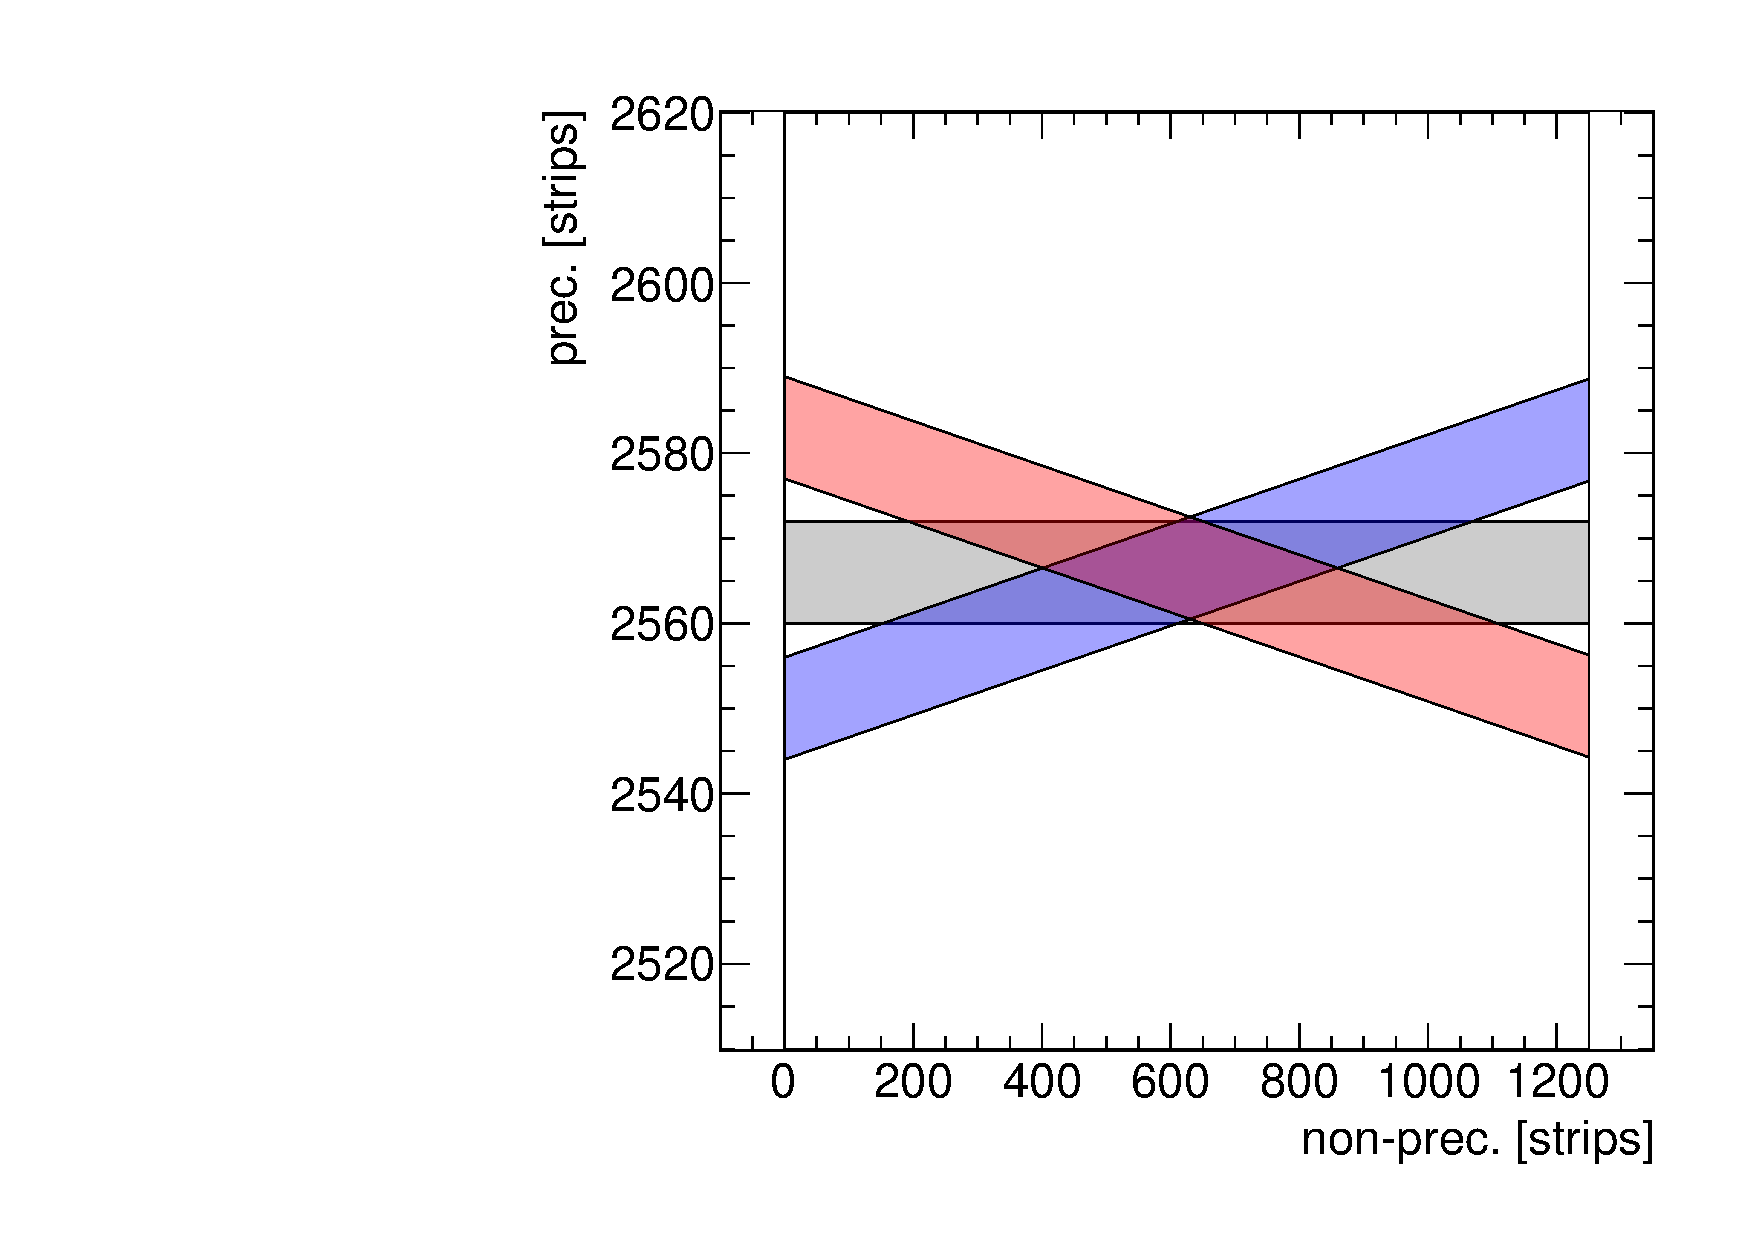
\includegraphics[width=0.48\textwidth]{figures/cartoon_roads_small_smallstereo_1.pdf}
    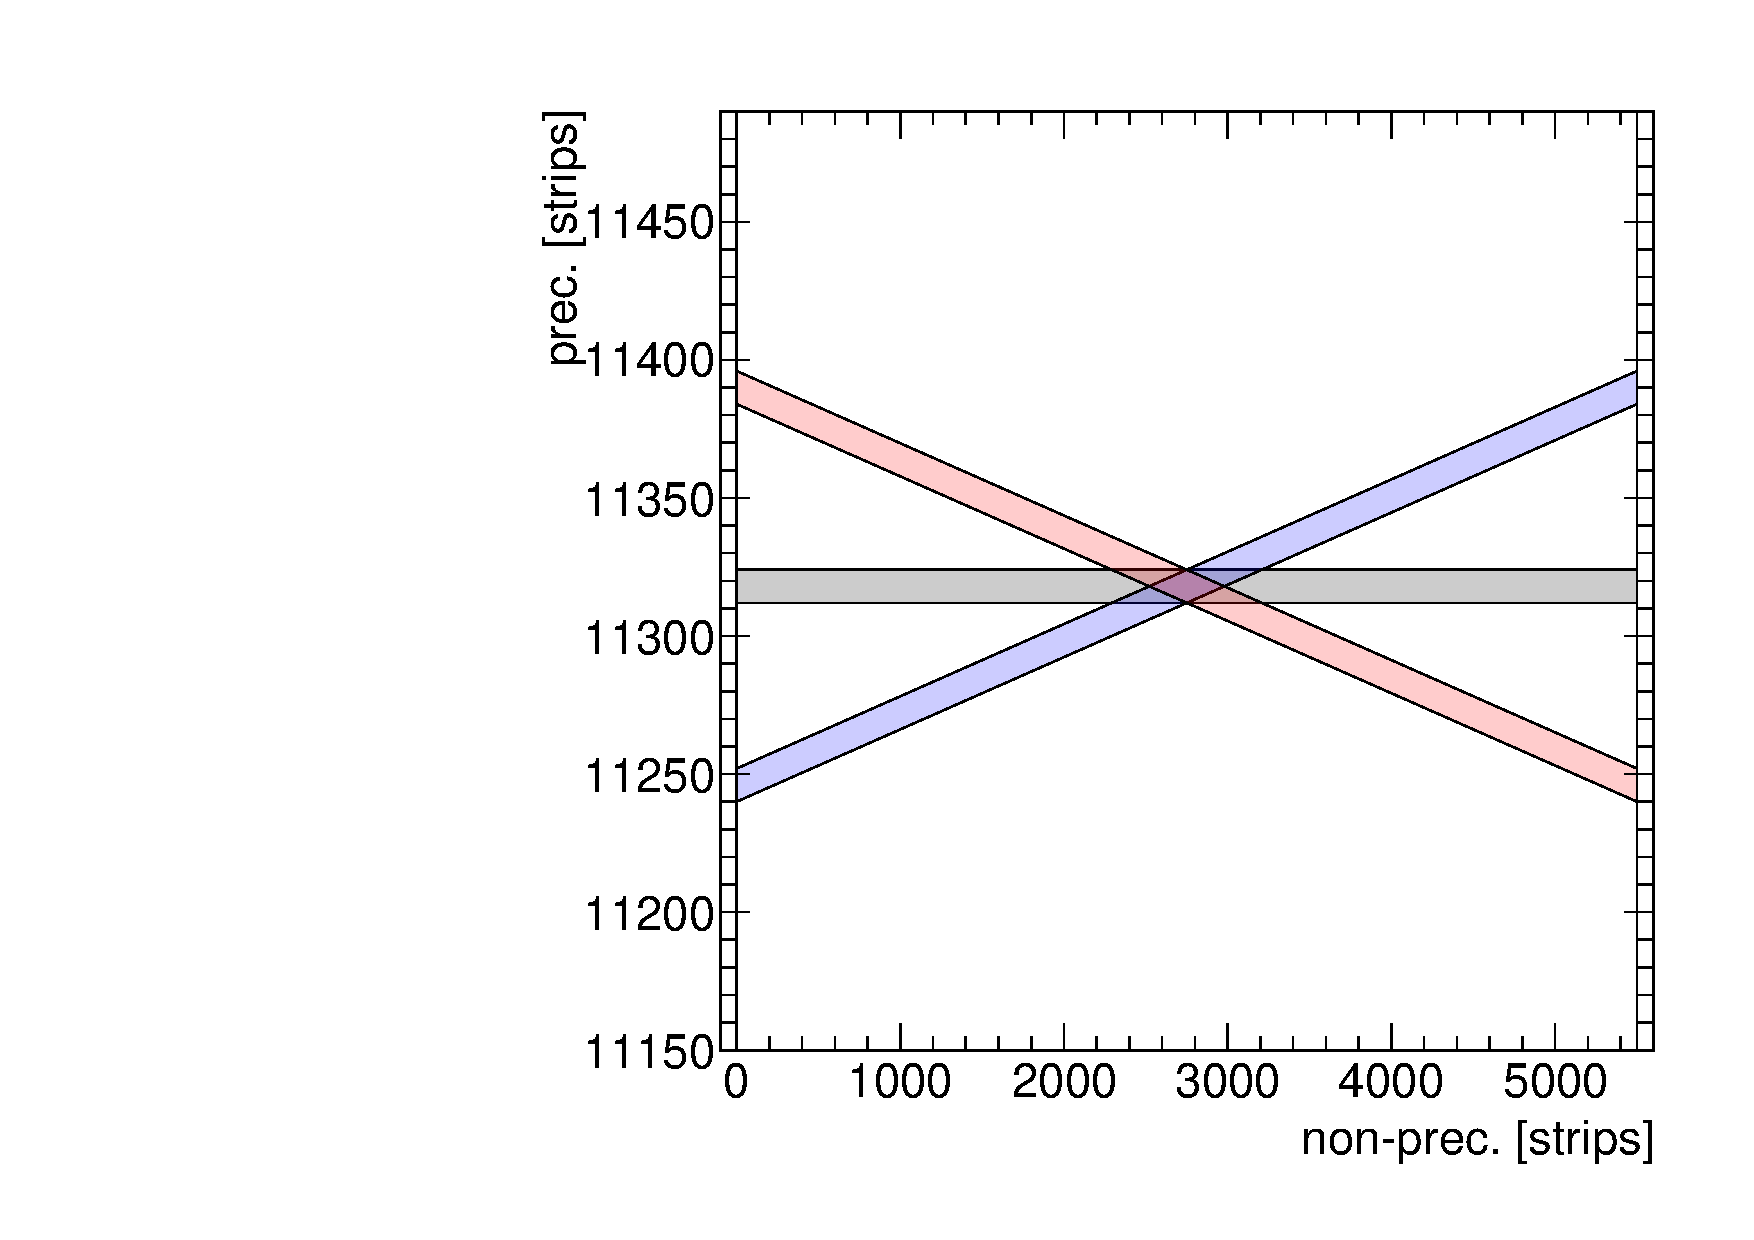
\includegraphics[width=0.48\textwidth]{figures/cartoon_roads_large_smallstereo_1.pdf}
  \end{center}
  \vspace{-10pt}
  \caption{Layout of the roads used by proposed MMTP algorithm, for a small chamber closest to the beamline (left)
 and large chamber farthest from the beamline (right). The X road is horizontal, the U road is pink and slanted,
 and the V road is blue and slanted. Only one pair of U and V roads is drawn, and  does not cover the entire length X road.
 The  $x$-axis (prec.) and $y$-axis (non-prec.) are in units of strip pitches, which are 0.4 mm.}
  \label{fig:cartoon_smallroads_1}
\end{figure}
%%%%%%%%%%%%%%%%%%%%%%%%%%%%%%%%%
%%%%%%%%%%%%%%%%%%%%%%%%%%%%%%%%%%
\begin{figure}[!htpb]
  \begin{center}
    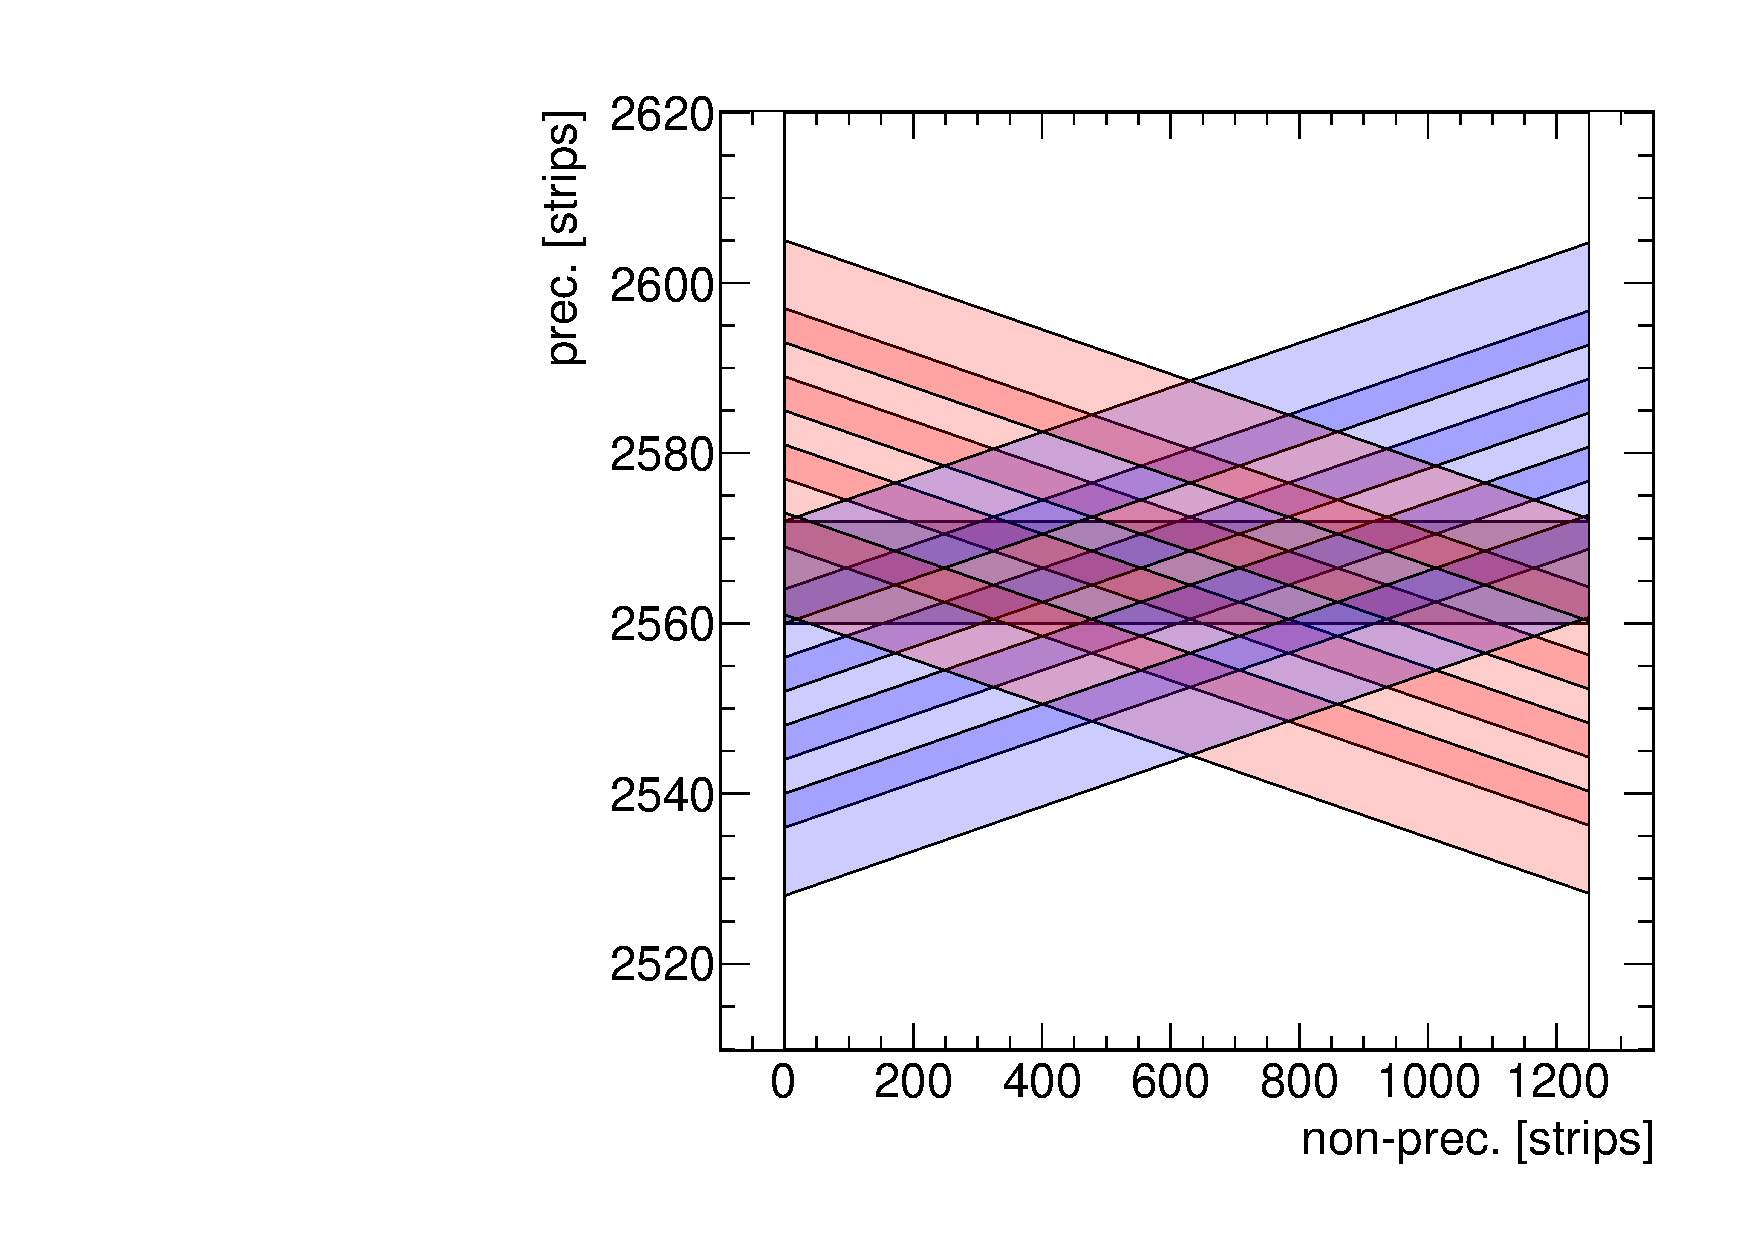
\includegraphics[width=0.48\textwidth]{figures/cartoon_roads_small_smallstereo_N.pdf}
    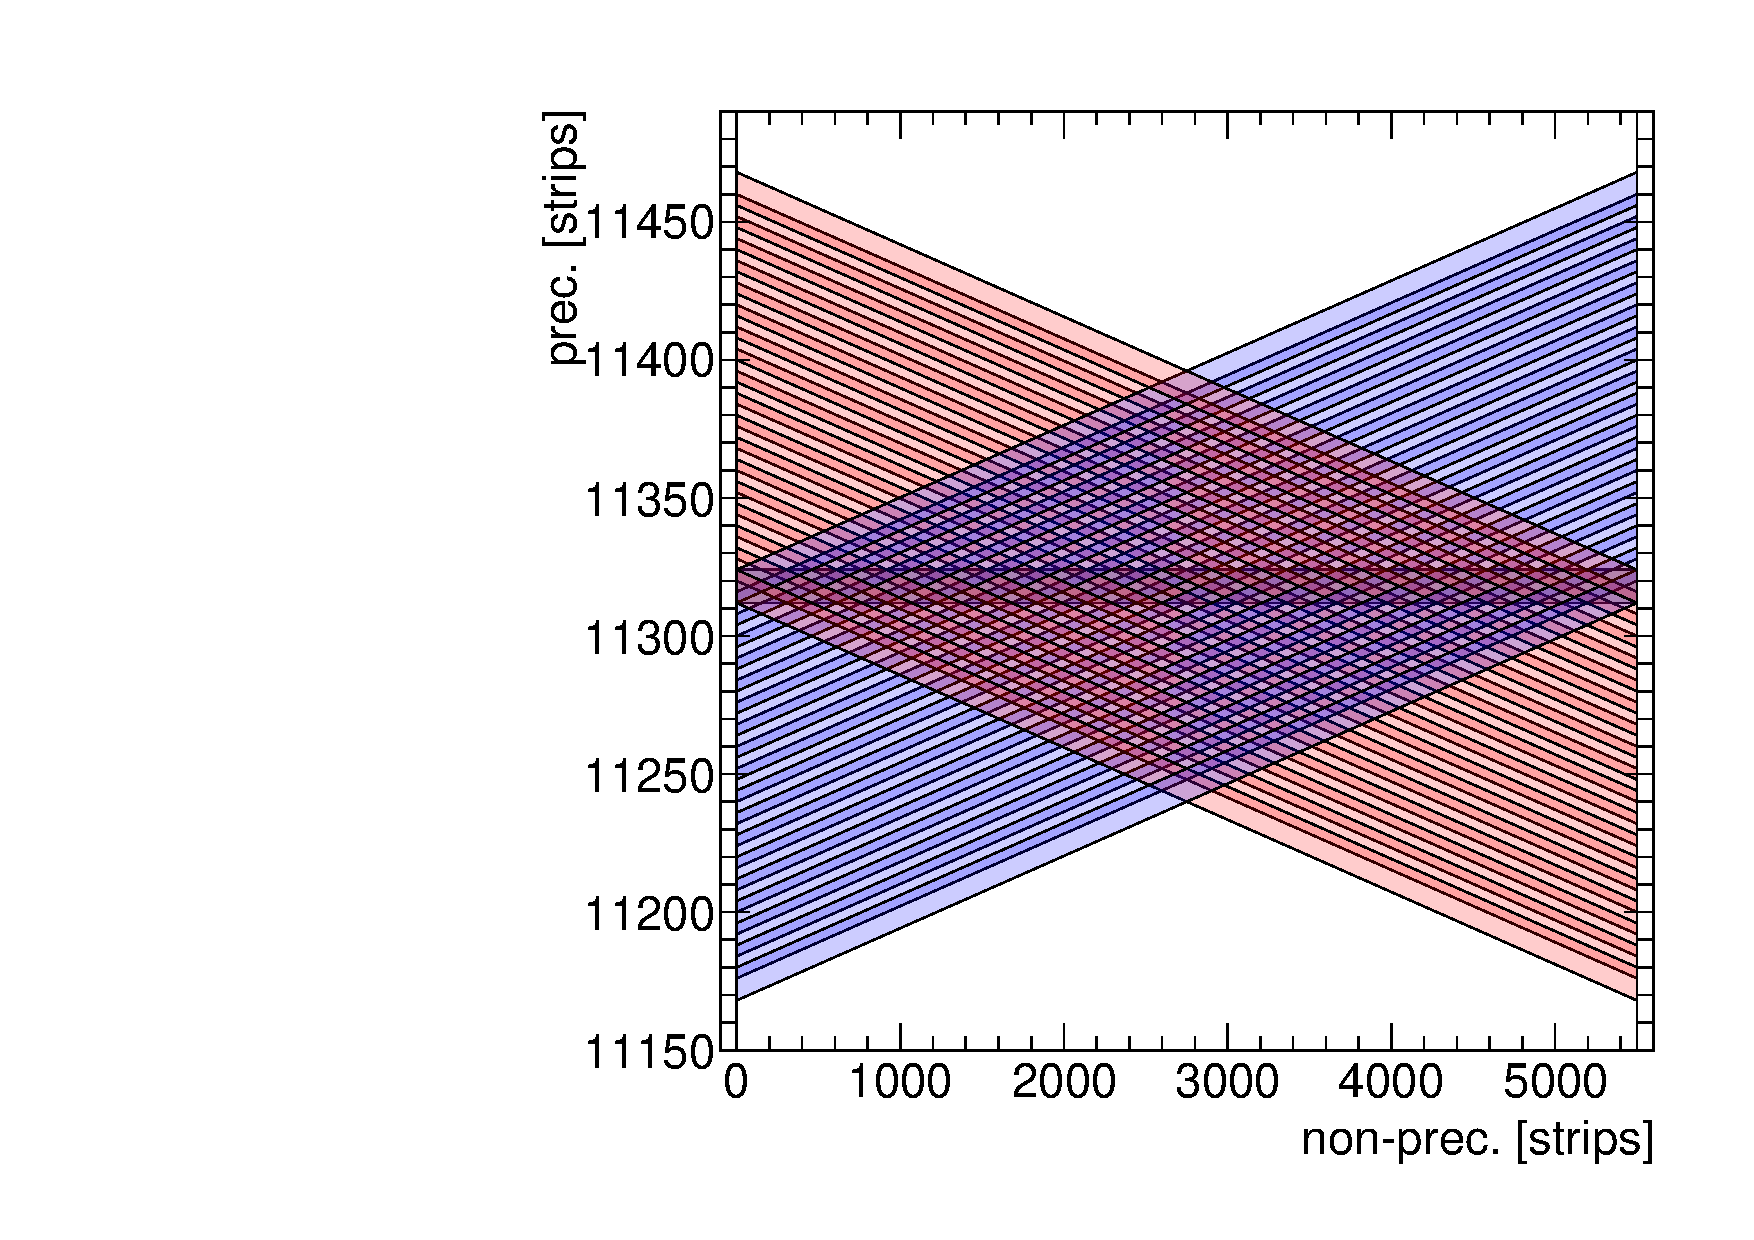
\includegraphics[width=0.48\textwidth]{figures/cartoon_roads_large_smallstereo_N.pdf}
  \end{center}
  \vspace{-10pt}
  \caption{Layout of the roads used by the proposed MMTP algorithm, for a small chamber closest to the beamline (left) and large chamber farthest
 from the beamline (right).The X road with shortest (longest) strips is covered with 5 (19) U and 5 (19) V roads.}
  \label{fig:cartoon_smallroads_N}
\end{figure}
%%%%%%%%%%%%%%%%%%%%%%%%%%%%%%%%%%%%%%%%%%%

 In the new algorithm, incoming hits are assigned to the respective X, U, and V roads with a maturity flag which expires after 8 (for now) BCs.  
 The  finder operates in two stages. In the first stage, the finder looks for any X road with at least 3 hits.
 If one such a road is found, in the second stage the finder enables a set of 4-fold majority AND-gates,
 one for each diamond overlapping the fired X road. The inputs
 of  each AND-gate corresponds to the four U,V roads defining the diamond and is set to 1 if a road has  one hit.
 If any of these coincidences has at least 3 U,V roads fired, a trigger is generated.
 This dramatically narrows the spatial region in which a coincidence is found.

\par The performance of the improved algorithm is illustrated by Figs.~\ref{fig:resolutions_new} and~\ref{fig:rms_vs_rate}. 
As expected, the $x$ resolution
 is comparable to that of the nominal algorithm that was already satisfactory. The $y$ resolution is much improved. 
Retaining as usual 99.7\% of the events, the rms value of the distribution is 11.22 (11.74) $\pm$ 0.01 (0.01) mm
 for 0.5 m (2.2 m) long strips.
%%%%%%%%%%%%%%%%%%%%%%%%%%%%%%%%%%%%%%%%%%%%%%%%%
\begin{figure}[!htpb]
  \begin{center}
    \includegraphics[width=0.48\textwidth]{figures/xres_new.pdf}
    \includegraphics[width=0.48\textwidth]{figures/yres_new.pdf}
    \includegraphics[width=0.48\textwidth]{figures/mres_new.pdf}
  \end{center}
  \vspace{-10pt}
  \caption{Distribution of $x_\text{reco.} - x_\text{truth}$ (top, left), $y_\text{reco.} - y_\text{truth}$ (top, right),
 and $\theta_\text{reco.} - \theta_\text{truth}$ (bottom)
 for the proposed MMTP algorithm in the presence of  uncorrelated background with a rate of 40 kHz per strip.
 This figure should be compared to Fig.~\ref{fig:resolutions_old}. }
  \label{fig:resolutions_new}
\end{figure}
%%%%%%%%%%%%%%%%%%%%%%%%%%%%%
%%%%%%%%%%%%%%%%%%%%%%%%%%%%
\begin{figure}[!htpb]
  \begin{center}
    \includegraphics[width=0.48\textwidth]{figures/rms_y_small_vs_rate.pdf}
    \includegraphics[width=0.48\textwidth]{figures/rms_y_large_vs_rate.pdf}
  \end{center}
  \vspace{-10pt}
  \caption{Dependence of rms value of $y_\text{reco.} - y_\text{truth}$  on
 the uncorrelated background rate for a strip length of (left) 0.5 m  and (right)  2.2 m.
 The rms is calculated  after a cut selecting 99\% of the events. This figure compares the performance of the nominal
and diamond-based algorithm.}
  \label{fig:rms_vs_rate}
\end{figure}
%%%%%%%%%%%%%%%%%%%%%%%%%%%%%%%%%%%%%%%%%%%%%
% We can also look at the efficiency of a $\Delta \phi <$ 20 mrad cut as a function of the uncorrelated background rate for both algorithms.
% In Figure \ref{fig:eff_vs_rate}, we see that the performance of the nominal algorithm drops sharply with increased background, 
%while the proposed algorithm maintains 80\% (95\%)+ efficiency for up to a 60 kHz/strip background rate with 0.5m (2.2m) long strips.
%\par We now elaborate on the use of implementation regions. It is important to divide the wedge into reasons so that each 
%implementation of the firmware has a minimum number of triggers to process at any given time. There will be hard limit to
% how many triggers can be processed per BC per implementation. Thus, small implementation regions are ideal. As a technical aside,
% the exact number of roads in an implementation region is presently determined by the architecture of
% the MMTP firmware. \footnote{The MMTP relies on multiplexers to select the $U$,$V$ roads overlapping with
% each $X$ road. If we consider the LM2 with a pitch of 450 microns,
% we have $2.2\text{m} \times \tan 1.5^\circ \times \frac{1}{450 \;\mu m \times 8 \text{ strips/road}} = 16 + 1$ $U$,$V$ roads associated
% to one $X$ road, so we need 17 multiplexers. Assuming standard multiplexer of 8:1, we can have 136 $X$ roads in the largest
% R region. A similar calculation can be done for the 0.5m strips.} 
%|begin{figure}[!htpb]
%  \begin{center}
%    \includegraphics[width=0.48\textwidth]{figures/eff_phi_small_vs_rate.pdf}
%    \includegraphics[width=0.48\textwidth]{figures/eff_phi_large_vs_rate.pdf}
%  \end{center}
%  \vspace{-10pt}
%  \caption{Efficiency of $\phi_\text{reco.} - \phi_\text{truth} < 20$ mrad for a strip size of 0.5m (left) and 2.2m (right).
% $\phi_\text{reco.}-\phi_\text{truth}$ is calculated as $\frac{y_\text{reco.} - y_\text{truth}}{R}$, where $R$ is the distance
% from the beamline. $R$ is taken to be 1m for the small chamber and 4.5m for the large chamber.}
%  \label{fig:eff_vs_rate}
%\end{figure}


% \input{tex/performance}
\section{Conclusions}
\label{sec:conclusion}

We have taken an upgraded MMTP algorithm from conception to the real world.



\clearpage

\begin{thebibliography}{99}
\label{bibliography}
\setlength{\itemsep}{1.5pt plus 2.0pt minus 1.4pt}
\setlength{\parsep}{0pt}
\setlength{\parskip}{0pt}
\vspace{-6pt}
\bibitem{nswtdr} ATLAS New Small Wheel Technical Design Report. \href{http://cds.cern.ch/record/1552862}{\color{blue}\underline{ATLAS-TDR-020}}.
 \href{https://cds.cern.ch/record/2272355}{\color{blue}\underline{ATL-COM-MUON-2017-036}}.
\bibitem{brian} B.~Clark {\it et al,} An Algorithm for Micromegas Segment
 Reconstruction in the Level-1 Trigger of the New Small Wheel. 
\href{https://cds.cern.ch/record/1706160}{\color{blue}\underline{ATL-COM-UPGRADE-2014-012}}.
\bibitem{steve} S.~Chan et. al. Micromegas Trigger Processor Algorithm Performance in Nominal, Misaligned, and Misalignment
 Corrected Conditions. \href{https://cds.cern.ch/record/2113121}{\color{blue}\underline{ATL-COM-UPGRADE-2015-033}}.
\bibitem{noisy} P.~Giromini {\it et al,} Performance of a Micromegas octuplet in the time  of noise.
 \href{https://cds.cern.ch/record/2277316}{\color{blue}\underline{ATL-COM-MUON-2017-036}}.
\bibitem{noiseless} P.~Giromini  {\it et al,} Performance of a Micromegas octuplet after removing the major cause of noise.
 \href{https://cds.cern.ch/record/2277316}{\color{blue}\underline{ATL-COM-MUON-2017-040}}.
\bibitem{mmtp} J. ~Farah {\it et al,} Test of the Micromegas Trigger Processor with Cosmic Ray Muons.
\bibitem{tuna} A. N. Tuna. Studies of the ATLAS MDT and CSC hit rates using proton-proton collisions at 13 TeV. 
  \href{https://cds.cern.ch/record/2111365}{\color{blue}\underline{ATL-COM-MUON-2015-098}}.
\bibitem{tpsim} N.~Felt \it et al,} Diamond-paved roads and steaming soup: the architecture of an upgraded Micromegas trigger processor and its optimization tool.
  \href{https://cds.cern.ch/record/2302523}{\color{blue}\underline{ATL-COM-MUON-2018-003}}.
\bibitem{phase2} ATLAS Muon Spectrometer Phase-II Upgrade Technical Design Report.
 \href{https://cds.cern.ch/record/2270169/}{\color{blue}\underline{ATL-COM-MUON-2017-033}}.
\bibitem{utpc} 
%\bibitem{oldart} K.~DiPetrillo  {it et al,} ATL-COM-MUON-2014-069.
%\bibitem{koki} Simulation of the ATLAS New Small Wheel (NSW) System
% \href{http://cds.cern.ch/record/2265067}{\color{blue}\underline{ATL-MUON-SLIDE-2017-248}}.
%\bibitem{lhc} LHC Design Report. 
% \href{https://cds.cern.ch/record/782076}{\color{blue}\underline{CERN-2004-003}}.

\end{thebibliography}










\end{document} 

